 %{{{ Preamble
\documentclass[a4paper,10pt]{article}
\usepackage{anysize}
\marginsize{2cm}{2cm}{1cm}{1cm}
%\textwidth 6.0in \textheight = 664pt
\usepackage{xltxtra}
\usepackage{graphicx}
\usepackage{subfig}
\usepackage{color}
\usepackage{xgreek}
\usepackage{framed}
\usepackage{float}
\usepackage{tkz-graph}
\setmainfont[Mapping=TeX-text]{CMU Serif}

%\setmainfont{Arial}
%\setsansfont{FreeSans}
%\setmonofont{FreeMono}
\begin{document}
\def\thesection {Άσκηση \arabic{section}}
\def\thesubsection {\roman{subsection})}
\def\thesubsubsection {(\arabic{subsubsection})}
%\renewcommand{\labelenumi}{\roman{enumi})}
\renewcommand{\labelenumi}{(\arabic{enumi})}
\renewcommand{\labelenumii}{(\arabic{enumii})}
%}}}
%{{{ Titlepage
\begin{titlepage}
\begin{center}
\begin{figure}[t] 
     
\includegraphics[scale=0.7]{title/ntua_logo}
\end{figure}
\begin{LARGE}\textbf{ΕΘΝΙΚΟ ΜΕΤΣΟΒΙΟ ΠΟΛΥΤΕΧΝΕΙΟ\\}\end{LARGE}
\vspace{5cm}
\begin{Large}
ΣΧΟΛΗ ΗΜ\&ΜΥ\\
Βάσεις Δεδομένων\\
2\textsuperscript{η} Σειρά Γραπτών Ασκήσεων\\
Ακ. έτος 2010-2011\\
\end{Large}
\vfill
\begin{flushright}
\Large{Λύρας Γρηγόρης}\\
\large{Α.Μ.: 03109687}\\
\end{flushright}
\large\today\\
\end{center}
\end{titlepage}


%}}}
%{{{ Άσκηση 1
\section{}
\noindent Αρχικό B+ δέντρο. Καλούμαστε να διαγράψουμε το 43.
\begin{figure}[h]
	\centering
	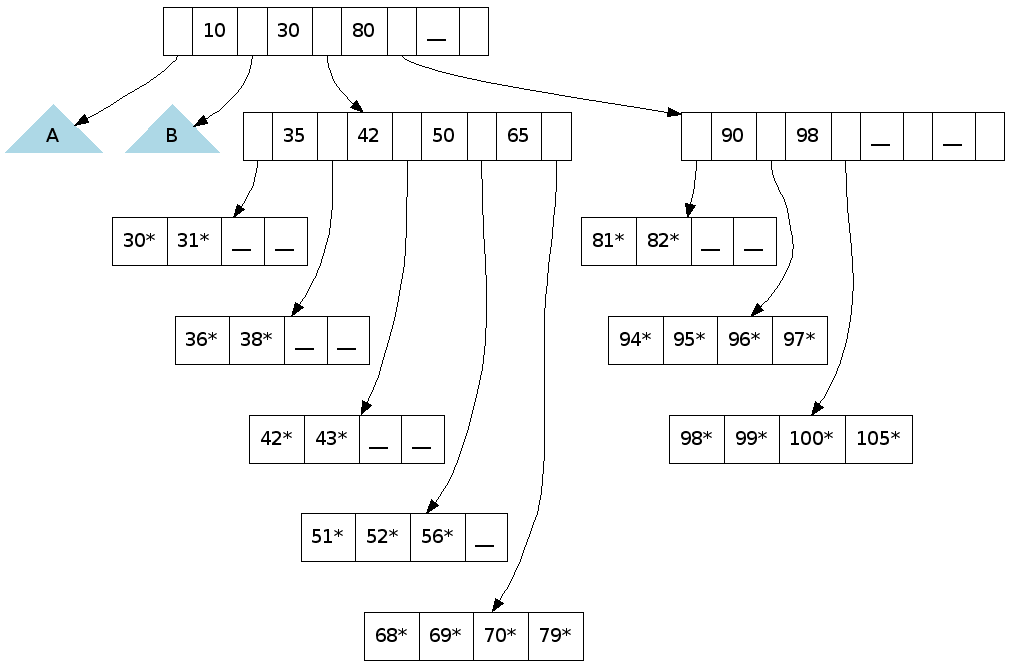
\includegraphics[width=0.7\textwidth]{files/init_tree.png}
\end{figure}

\subsection{Καινούρια B+ δέντρα}
		\begin{enumerate}
			\item
				Κάνοντας συγχώνευση του φύλλου με το δεξιό αδελφό του
				\begin{figure}[H]
					\centering
					\includegraphics[width=0.7\textwidth]{files/tree1a.png}
				\end{figure}
				\pagebreak
			\item
				Κάνοντας συγχώνευση του φύλλου με τον αριστερό αδελφό του
				\begin{figure}[H]
					\centering
					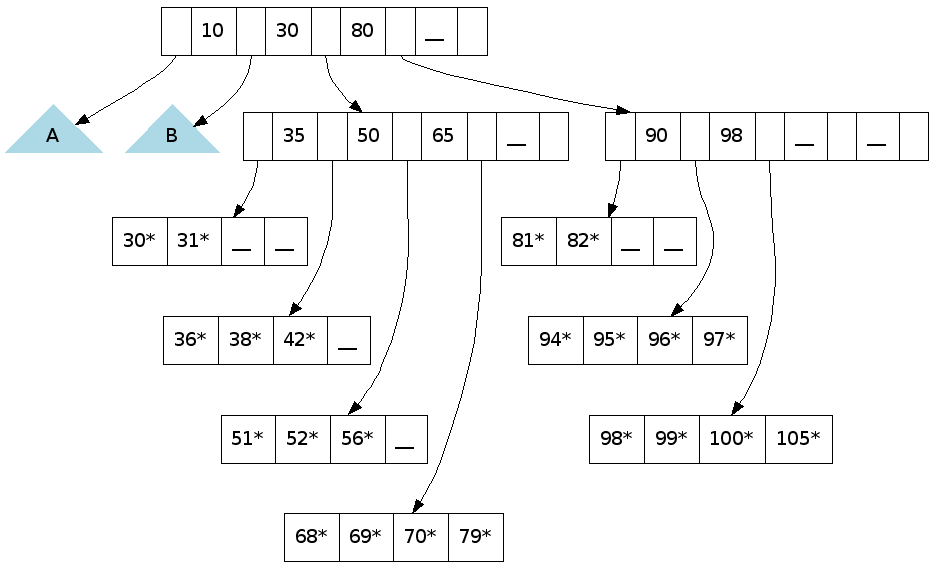
\includegraphics[width=0.7\textwidth]{files/tree1b.png}
				\end{figure}
			\item
				Κάνοντας ανακατανομή των εγγραφών του φύλλου με το δεξιό αδελφό του
				\begin{figure}[H]
					\centering
					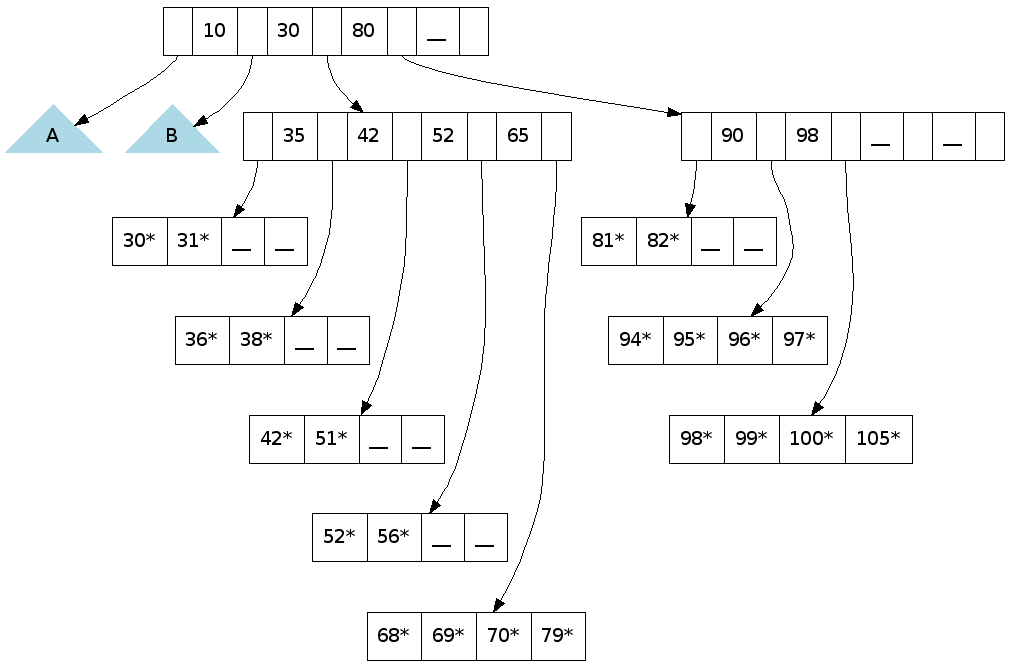
\includegraphics[width=0.7\textwidth]{files/tree1c.png}
				\end{figure}
		\end{enumerate}
\subsection{Κόστος}
Το χαμηλότερο κόστος το έχει η ανακατανομή των εγγραφών καθώς το μόνο που
απαιτείται να κάνουμε είναι μεταφορά μιας εγγραφής στο ζητούμενο φύλλο και μια
αλλαγή στο κλειδί του κόμβου πατέρα (51->52) και αφήνει το δέντρο σε πιο
συμβατή κατάσταση με 3 minimal-sized φύλλα.
\subsection{Προτιμώμενη επιλογή}
Αν οι διαγραφές είναι πιο σπάνιες από τις εγγραφές τότε προτιμούμε να κάνουμε
ανακατανομή εγγραφών καθώς έτσι θα έχουμε τη δυνατότητα να εισάγουμε εγγραφές
πιο εύκολα στη συνέχεια. Αν όμως θέλουμε να κάνουμε συνεχώς διαγραφές η
συγχώνευση είναι προτιμότερη καθώς θα οδηγήσει σε μείωση των κλειδιών στον
πατέρα και θα μειώσει γρηγορότερα το ύψος του δέντρου.
\pagebreak
%}}}
%{{{ Άσκηση 2
\section{}
Για να είναι ισορροπημένο το παραπάνω δέντρο πρέπει τα Α και Β να έχουν ύψος
ίσο με 2 και για να είναι όσο το δυνατόν πιο άδεια θα πρέπει να έχουν
2 τιμές στο ευρετήριο άρα 3 φύλλα έκαστο και 2 κλειδιά σε κάθε φύλλο,
$2*3*2=12$ blocks δίσκου στα Α και Β, συνεπώς συνολικά $12+23=35$ blocks. Αν
σε κάθε block έχουμε 20 εγγραφές τότε $35*20=700$ πλειάδες.
%}}}
%{{{ Άσκηση 3
\section{Κόστος ερωτημάτων}
%{{{ Απευθείας προσέλαση
\subsection{Απευθείας προσπέλαση}
\subsubsection{$\sigma_{A < 60000}$}
Θα πρέπει να προσπελαστούν όλες οι εγγραφές μέχρι 60000. Με δεδομένο πως κάθε
block χωράει 10 εγγραφές θα μεταφερθούν $60000/10=6000$ blocks στη μνήμη άρα
το κόστος είναι 6000 I/O.
\subsubsection{$\sigma_{A = 60000}$}
Εφόσον το αρχείο είναι διατεταγμένο σε αύξουσα σειρά μπορούμε να κάνουμε
δυαδική αναζήτηση και να βρούμε το block που ζητάμε με λογαριθμικό κόστος
$log_2{(6000000)} \simeq 23$ I/O.
\subsubsection{$\sigma_{A\; >\; 60000\; AND\; A\; <\; 60010}$}
Εδώ επίσης σειρά μπορούμε να κάνουμε δυαδική αναζήτηση και να έχουμε
λογαριθμικό κόστος $log_2{(6000000)} \simeq 23$ I/O και στη συνέχεια να
προχωρήσουμε σειριακά μέχρι να ξεπεράσουμε το όριο με κόστος $1$ συνεπώς
συνολικά $24$ I/O.
\subsubsection{$\sigma_{A <> 60000}$}
Θα πρέπει να προσπελάσουμε όλο το αρχείο συνεπώς το κόστος είναι
$6000000/10=600000$ I/O.
%}}}
\subsection{Με χρήση B+ δέντρου}
\subsubsection{$\sigma_{A < 60000}$}
Για να κάνουμε αναζήτηση στο δέντρο θα χρειαστούμε 4 I/O για να φτάσουμε στο
πρώτο φύλλο και στη συνέχεια να φέρουμε τα επόμενα 600 τα οποία με τη σειρά
τους θα φέρουν τα blocks που περιέχουν τις εγγραφές που χρειαζόμαστε. Συνολικά
$4+600+6000=6604$ I/O.
\subsubsection{$\sigma_{A = 60000}$}
Με κόστος 4 I/O μπορούμε να βρούμε το φύλλο που περιέχει την πληροφορία για το
ζητούμενο block και με άλλο 1 I/O θα έχουμε την πληροφορία στη μνήμη. Συνολικά
4 I/O.
\subsubsection{$\sigma_{A > 60000 AND A < 60010}$}
Με κόστος 4 I/O μπορούμε να φτάσουμε στο φύλλο που περιέχει πληροφορία για το
πρώτο block και με άλλα 2 I/O θα έχουμε τις εγγραφές αυτού και του επόμενού
του στη μνήμη. Συνολικά 6 I/O.
\subsubsection{$\sigma_{A <> 60000}$}
Θα πρέπει να φτάσουμε στο πρώτο φύλλο με κόστος 4 I/O και στη συνέχεια να
προσπελάσουμε όλα τα φύλλα με κόστος 60000 I/O και στη συνέχεια να φέρουμε
όλα τα blocks των εγγραφών από το δίσκο με κόστος 6000000 I/O. Συνολικά 660004
I/O.
\subsection{Με χρήση ευρετηρίου κατακερματισμού}
\subsubsection{$\sigma_{A < 60000}$}
Θα έχουμε κόστος 60000 I/O καθώς κάθε εγγραφή από αυτό το εύρος βρίσκεται σε
διαφορετικό block με χρήση κατακερματισμού.
\subsubsection{$\sigma_{A = 60000}$}
Το κόστος εδώ είναι 1 I/O μιας και η συνάρτηση κατακερματισμού θα μας δείξει
κατευθείαν σε ποιο block βρίσκεται το αρχείο μας.
\subsubsection{$\sigma_{A > 60000 AND A < 60010}$}
Το κόστος είναι 10 I/O καθώς για κάθε εγγραφή στο διάστημα 60000-60010 θα
πρέπει να ανακτήσουμε διαφορετικό block από το δίσκο.
\subsubsection{$\sigma_{A <> 60000}$}
Το κόστος εδώ είναι 600000 I/O μιας και ζητάμε όλες τις εγγραφές εκτός από
μία.
%}}}
%{{{ Άσκηση 4
\section{}
\subsection{}
Αν δεν υπάρχουν υπερχειλίσεις τότε το αρχείο αποθηκεύεται σε 1000 blocks στο
δίσκο.
\subsection{}
Η σχέση αυτή δεν χωράει σε λιγότερα από 1000 blocks.
\subsection{}
Σε αυτή την περίπτωση θα είχαμε και υπερχείλιση συνεπώς θα χρειαζόμασταν 1000
blocks για τα 100000 πρώτα στοιχεία και άλλο 1 block για κάθε εγγραφή ακόμα
συνεπώς 1099 blocks.
%}}}
\end{document}
